\documentclass[12pt,a4paper,titlepage]{article}
\usepackage{mypack}
\usepackage{fancyhdr}
\usepackage{imakeidx}

\newcommand{\course}{Cálculo Numérico}
\newcommand{\semester}{12/13 C2}


\newcommand{\subject}{Análisis de requisitos}
\newcommand{\nombre}{Víctor de Juan Sanz - Guillermo Julián Moreno}
\makeindex
\fancyhf{}


\fancypagestyle{plain}{%
\lhead{\itshape \subject}
\rhead{\nombre}
\cfoot{\thepage\ de \pageref{LastPage}}}

%
\author{Víctor de Juan Sanz - \emph{vic.juan@estudiante.uam.es}  \\ Guillermo Julián Moreno - \emph{guillermo.julian@estudiante.uam.es}}
\date{Febrero 2013}
\title{Documento de análisis de requisitos}
%

\makeindex

\begin{document}

\pagestyle{plain}
\maketitle
\newpage

\tableofcontents
\newpage
\section{Introducción}
\subsection{Propósito del sistema}

El cliente demanda una aplicación para gestionar las compras, reservas y cancelaciones de viajes organizados, vuelos y hoteles.
\subsection{Ámbito del sistema}

El sistema debe permitir la venta de hoteles, vuelos y viajes organizados disponibles. Así mismo, deberá permitir la gestión de las reservas dentro del sistema y de los métodos de pago (no se incluye la gestión de la reserva con los agentes externos: aerolíneas, hoteles, etc).

Además, debe existir un rol de administrador que puede obtener reportes y estadísticas de los beneficio y productos vendidos, tanto de los vendedores individuales como de toda la agencia en conjunto.

El vendedor deberá entrar en el sistema con su cuenta antes de poder ejecutar ninguna acción. Una vez en su cuenta, al llegar un cliente, la aplicación le dará de alta guardando nombre, apellido y DNI (si no está ya registrado como cliente). El vendedor puede vender tres tipos de productos: hotel, vuelo y viajes organizados, formalizar los pagos y 


\subsection{Objetivos y criterios de éxito del proyecto}

Conseguir una funcionalidad del sistema acorde con los requisitos del cliente y sin presentar dificultades para el usuario, tanto desde el punto de vista del rendimiento del sistema como de la usabilidad. El objetivo es facilitar el trabajo de los vendedores y por ello deberemos procurar que nuestra aplicación tenga una curva de aprendizaje muy rápida.

\subsection{Definiciones, acrónimos y abreviaturas}

Lista con términos técnicos y abreviaturas que se usarán en el resto del documento.

\begin{description}
\item[Servicio] Hotel, vuelo o viaje organizado. Lo proveen entidades externas a la agencia.
\item[Cliente] Persona que contrata los servicios de vuelo, hotel o viaje organizado a través de la agencia.
\item[Usuario] Persona que usa nuestra aplicación, ya sea cliente o vendedor.
\item[Login] Nombre de usuario que identifica a un vendedor o administrador en el sistema. Es único para cada usuario.
\item[Contraseña] Código que permite el acceso de un usuario al sistema. Las contraseñas se guardan de forma segura (\textit{hash+salt}) en la base de datos de la aplicación.
\item[Base de datos] El sistema guardará todos los datos en una base de datos. Será un archivo SQLite embebido en la aplicación.
\item[SQL] Structured Query Language, lenguaje de acceso y consulta a bases de datos. Será la interfaz que usemos entre la aplicación y la base de datos del sistema.
\end{description}

\section{Descripción del sistema}

\subsection{Requisitos funcionales}

Pasamos a describir los dos tipos de usuario del sistema y los requisitos que tiene cada uno de ellos.

\subsubsection{Vendedor}

El vendedor entra con su cuenta (usuario/contraseña) en el sistema. Además, debe poder realizar las siguientes acciones sobre cada elemento del sistema:

\paragraph{Clientes}
\begin{itemize}
\item La aplicación tiene que mantener un registro de clientes que el vendedor puede consultar.
\item De cada cliente, se almacena el nombre, apellidos y DNI. Si además el cliente es de la tercera edad, se registrará también el número de Seguridad Social y fecha de nacimiento.
\end{itemize}

\paragraph{Paquetes}
\begin{itemize}
\item Los paquetes son conjuntos de reservas.
\item Las reservas sólo se pueden gestionar dentro de los paquetes.
\item El vendedor debe poder abrir y cerrar paquetes, y añadir y cancelar reservas.
\item El paquete se cierra automáticamente el día en el que empieza el primer servicio.
\item Si al momento del cierre del paquete hay reservas que no han sido pagadas por completo, se cancelarán.
\end{itemize}


\paragraph{Hoteles}

\begin{itemize}
\item La aplicación tiene que realizar búsquedas en un único catálogo en el que se encuentra la información de los hoteles por precio y ciudad. 
\item Un mismo cliente podrá realizar una reserva para varias personas a su nombre o a nombre de otra persona.
\item Se puede reservar pagando el 10\% del precio o pagando todo el coste de una vez.
\item En ningún momento se gestiona la reserva con el hotel, sólo se guarda la información de la reserva, quién la ha reservado y a nombre de quién está. También se almacena el método de pago: tarjeta o efectivo. No es necesario guardar el número de la tarjeta.
\end{itemize}

\paragraph{Vuelos}

\begin{itemize}
\item La aplicación será compatible con lo que recibiremos para realizar búsquedas de los vuelos y las plazas disponibles entre aeropuertos.
\item Se debe poder realizar una reserva: Esta reserva dura 2 días y es gratuita. Si al cabo de los dos días no ha sido confirmada se cancelará automáticamente.
\item Confirmar una reserva consiste en registrar que el cliente haya pagado el 100\% del precio de la reserva. Nuestra aplicación en ningún caso se encargará de gestionar la reserva en sí, simplemente guardará un registro con la información.
\item Se guardará la información personal (nombre, apellidos y DNI) de cada uno de los viajeros.
\item Se guardará también el método de pago del vuelo.
\end{itemize}

\paragraph{Viajes organizados}
\begin{itemize}
\item La aplicación buscará los viajes organizados en un catálogo dado.
\item Un viaje organizado es un conjunto de hoteles y viajes.
\item Se puede reservar pagando el 10\% del precio o pagando todo el coste de una vez.
\item El IMSERSO subvenciona los viajes a los clientes de la tercera edad. En este caso, habrá que introducir un código de descuento que dará la institución. La aplicación no verificará la validez del código.

\end{itemize}

\subsubsection{Administrador}

\begin{itemize}
\item El administrador deberá poder hacer todas las tareas de los vendedores.
\item El administrador es el gestor de usuarios de la aplicación: debe poder crear nuevas cuentas de vendedores y eliminarlas del sistema.
\item El administrador puede resetear las contraseñas de los vendedores.
\item La aplicación mostrará estadísticas de ventas globales y por vendedor.
\end{itemize}  
  
\subsection{Requisitos no funcionales}

\begin{itemize}
\item El sistema deberá notificar automáticamente si alguno de los paquetes está a un día de cerrarse y aún contiene servicios sin pagar.
\end{itemize}

\section{Casos de uso}
\subsection{Diagrama de casos de uso}
\easyimg{CasosUsoVendedor.png}{Casos de uso del vendedor}{imgCUVendedor}
\easyimg{CasosUsoAdmin.png}{Casos de uso del administrador. Además, el administrador puede hacer todas las tareas del vendedor}{imgCUAdmin}

\newpage
\subsection{Descripción de los casos de uso}
\subsubsection{Caso de uso: Añadir reserva a un paquete}
\begin{description}
\item[Actor Primario] Vendedor.
\item[Interesados y Objetivos] Cliente.
\item[Precondiciones] El vendedor ha creado un paquete abierto y localizado un servicio a reservar.
\item[Garantía de éxito (Postcondiciones)] La reserva se añade el paquete pagando el precio de reserva (10\% en hoteles y viajes, 0 en vuelos).
\item[Extensiones (Flujos alternativos)] El cliente paga el precio completo del servicio.
\item[Lista de variaciones de tecnología y datos] Una consulta SQL preparada para añadir nuevas reservas a la base de datos.
\item[Frecuencia de ocurrencia] Cinco veces al día.
\end{description}

\subsubsection{Caso de uso: Añadir cliente}
\begin{description}
\item[Actor Primario] Vendedor.
\item[Precondiciones] El vendedor tiene el nombre, apellidos y DNI del cliente, y no está registrado en el sistema.
\item[Garantía de éxito (Postcondiciones)] El cliente queda registrado en la base de datos.
\item[Lista de variaciones de tecnología y datos] Una consulta SQL preparada para añadir nuevos clientes a la base de datos.
\item[Frecuencia de ocurrencia] Cinco veces al día.
\end{description}

\subsubsection{Caso de uso: Ver estadísticas}
\begin{description}
\item[Actor Primario] Administrador.
\item[Precondiciones] El sistema está poblado con vendedores que ya han realizado reservas.
\item[Garantía de éxito (Postcondiciones)] El administrador obtiene las estadísticas detalladas de reservas realizadas y beneficios obtenidos en toda la agencia.
\item[Extensiones (Flujos alternativos)] El administrador puede obtener los mismos datos de un único vendedor.
\item[Lista de variaciones de tecnología y datos] Prepararemos una consulta SQL para extraer todos los datos de la base de datos.
\item[Frecuencia de ocurrencia] Una vez al día.
\end{description}

\section{Maquetas}

\begin{figure}[hbtp]   
	\begin{center} 
		\fbox{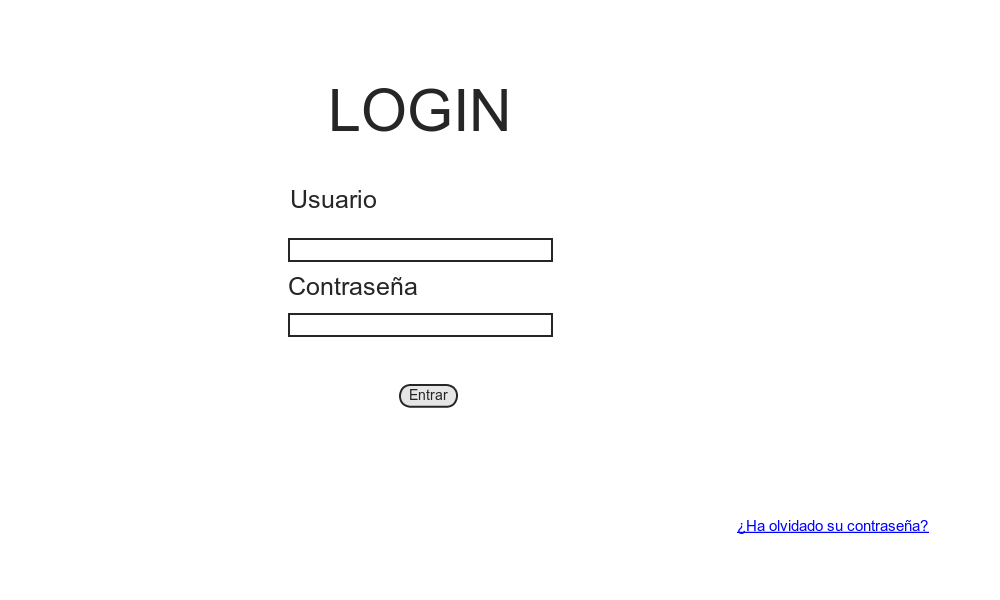
\includegraphics[width=0.8\textwidth]{Maquetas/Home.png}}
		\caption{Pantalla inicial: el usuario introduce su login y contraseña para usar la aplicación} 
	\end{center}  
\end{figure}
		
\begin{figure}[hbtp]   
	\begin{center} 
		\fbox{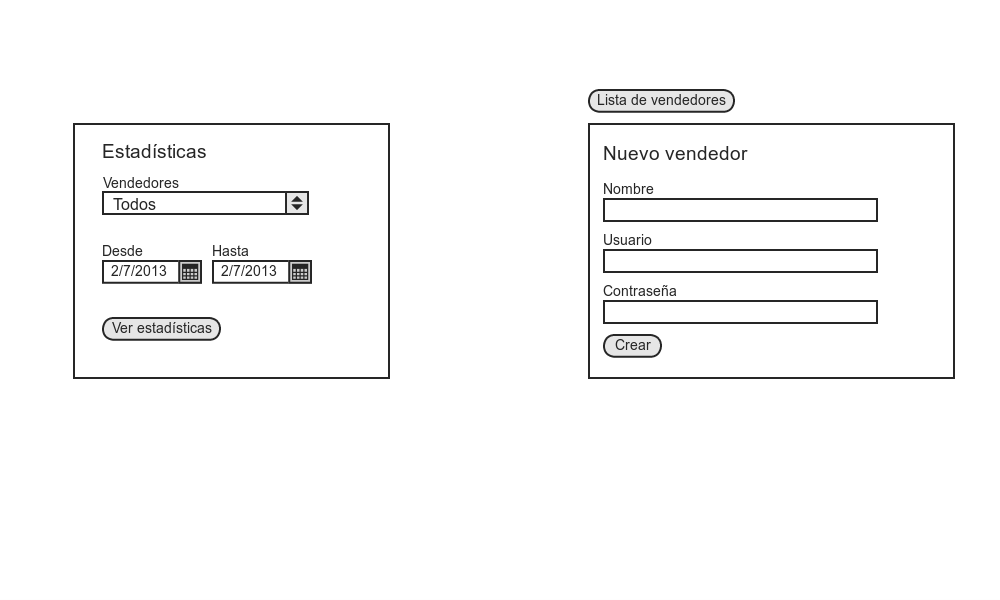
\includegraphics[width=0.8\textwidth]{Maquetas/Administrador.png}}
		\caption{Pantalla de administrador, con las funciones específicas de estadísticas y gestión de vendedores.} 
	\end{center}  
\end{figure}

\begin{figure}[hbtp]   
	\begin{center} 
		\fbox{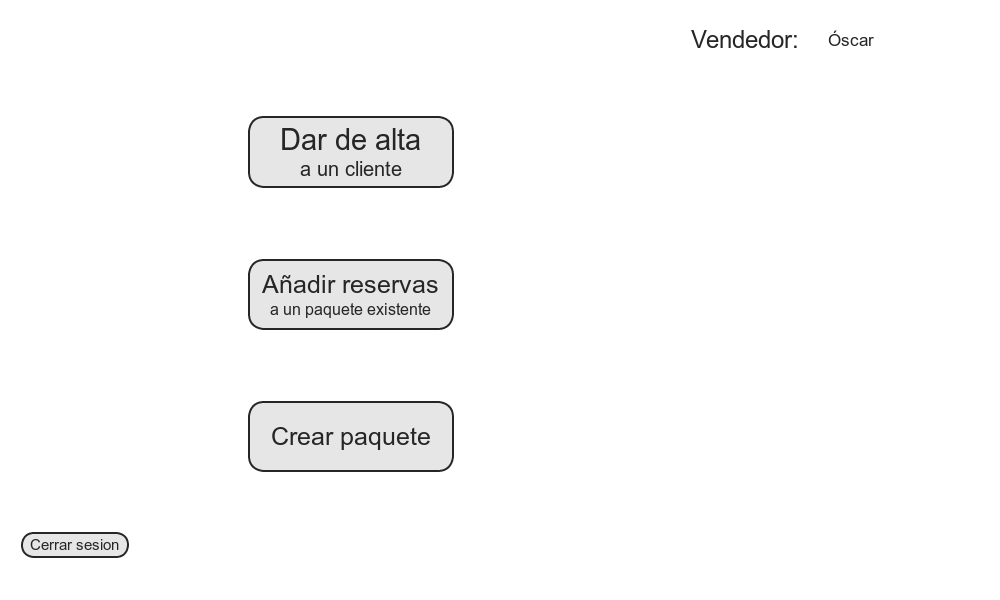
\includegraphics[width=0.8\textwidth]{Maquetas/Vendedor.png}}
		\caption{Pantalla de inicio del vendedor, desde donde puede navegar a las ventanas para hacer las distintas tareas del sistema.} 
	\end{center}  
\end{figure}

\begin{figure}[hbtp]   
	\begin{center} 
		\fbox{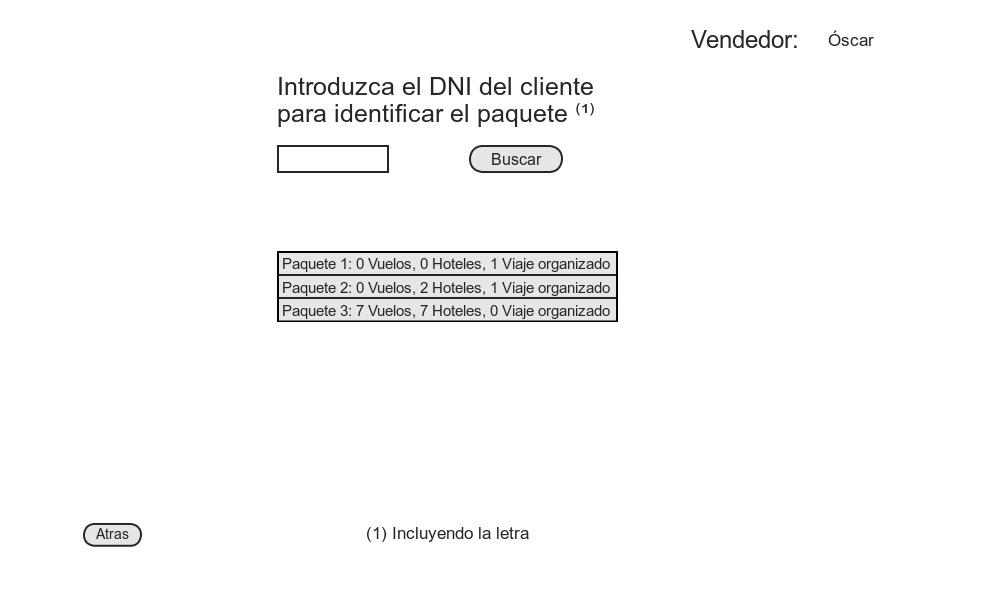
\includegraphics[width=0.8\textwidth]{Maquetas/BusquedaPaquete.png}}
		\caption{Desde aquí, el vendedor puede localizar los paquetes abiertos para cada cliente. En caso de que no exista, tendrá la opción de darle de alta (pantalla \ref{maqAltaCliente}).} 
	\end{center}  
\end{figure}

\begin{figure}[hbtp]   
	\begin{center} 
		\fbox{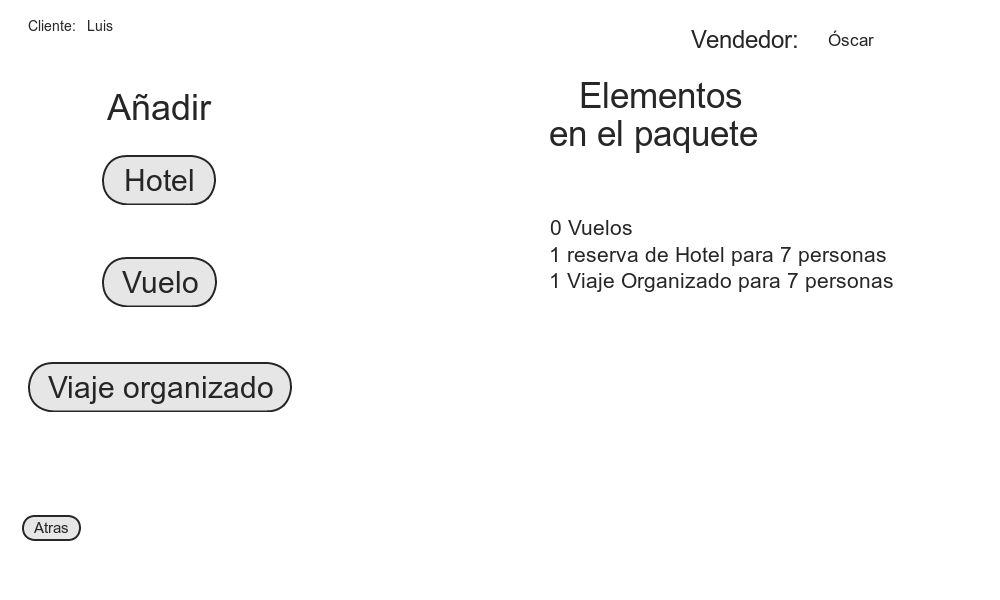
\includegraphics[width=0.8\textwidth]{Maquetas/Reservas.png}}
		\caption{La pantalla de reservas. Desde aquí se pueden añadir y eliminar reservas del paquete. La aplicación llevará a la pantalla de búsqueda correspondiente para localizar un vuelo (figura \ref{maqVuelo}), hotel (figura \ref{maqHotel}) o viaje organizado (figura \ref{maqOrganizado}). } 
	\end{center}  
\end{figure}

\begin{figure}[hbtp]   
	\begin{center} 
		\fbox{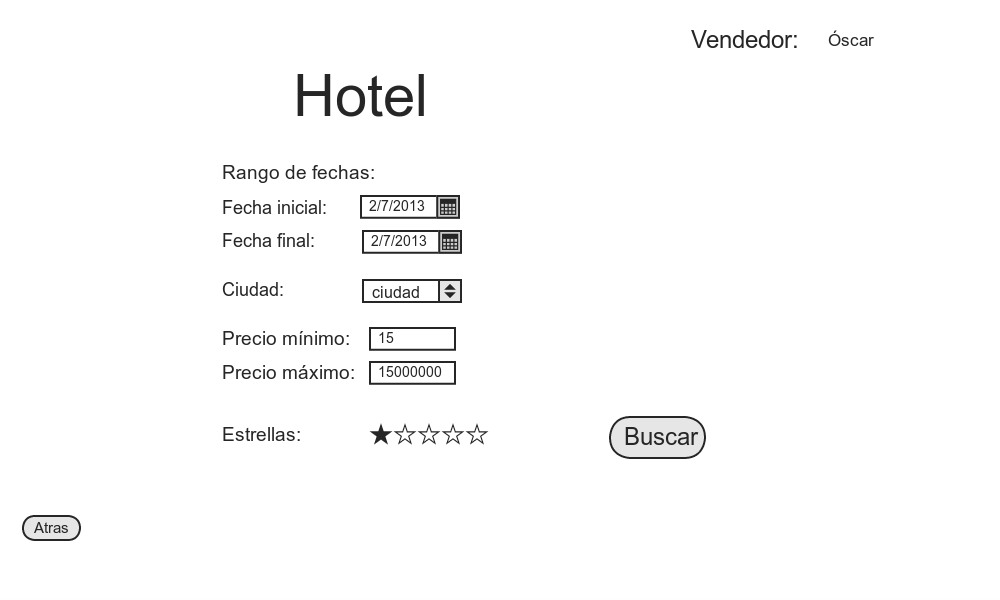
\includegraphics[width=0.8\textwidth]{Maquetas/Hotel.png}}
		\caption{Pantalla específica para buscar hoteles.} 
		\label{maqHotel}
	\end{center}  
\end{figure}

\begin{figure}[hbtp]   
	\begin{center} 
		\fbox{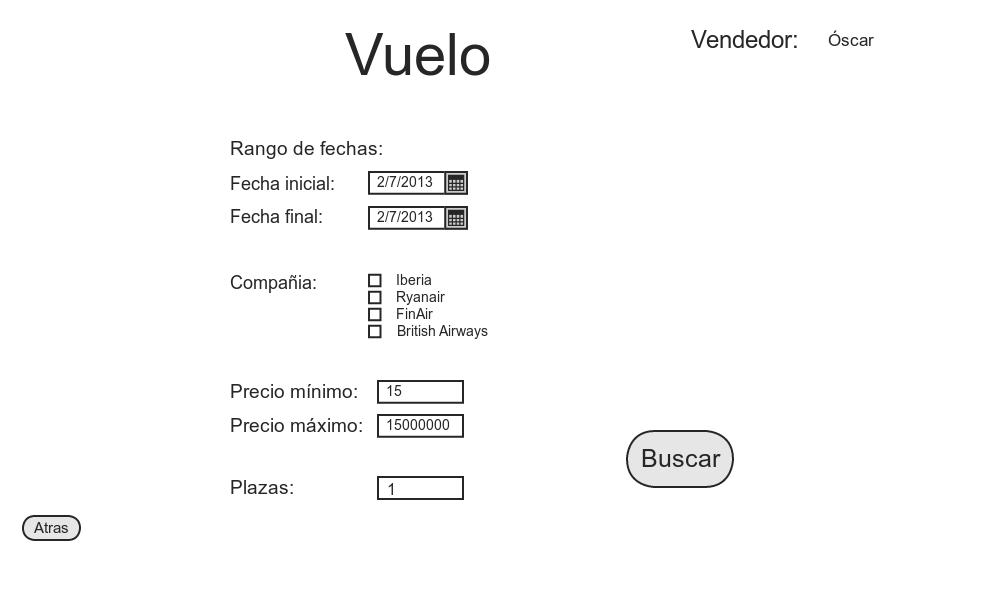
\includegraphics[width=0.8\textwidth]{Maquetas/Vuelo.png}}
		\caption{Pantalla específica para buscar vuelos.} 
		\label{maqVuelo}
	\end{center}  
\end{figure}

\begin{figure}[hbtp]   
	\begin{center} 
		\fbox{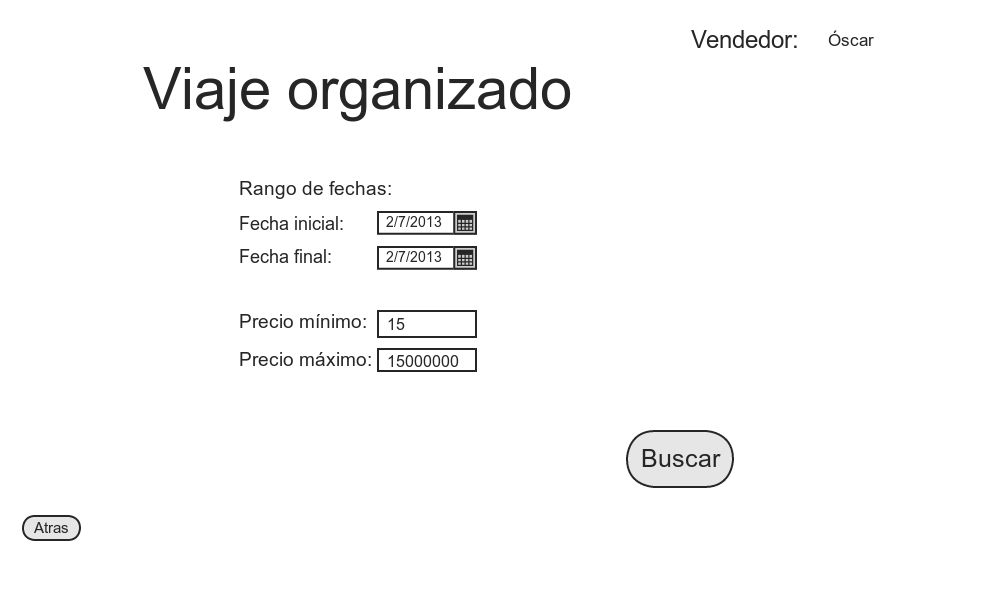
\includegraphics[width=0.8\textwidth]{Maquetas/Organizado.png}}
		\caption{Pantalla específica para buscar viajes organizados.} 
		\label{maqOrganizado}
	\end{center}  
\end{figure}

\begin{figure}[hbtp]   
	\begin{center} 
		\fbox{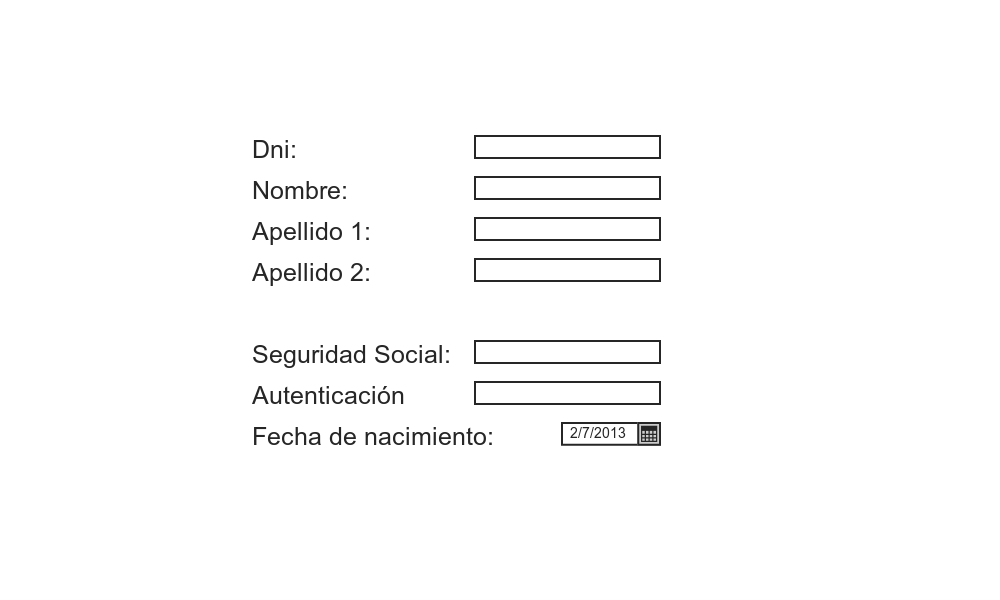
\includegraphics[width=0.8\textwidth]{Maquetas/DoReserva.png}}
		\caption{Pantalla para realizar la reserva de un servicio, que aparece una vez se ha seleccionado un servicio.} 
	\end{center}  
\end{figure}

\begin{figure}[hbtp]   
	\begin{center} 
		\fbox{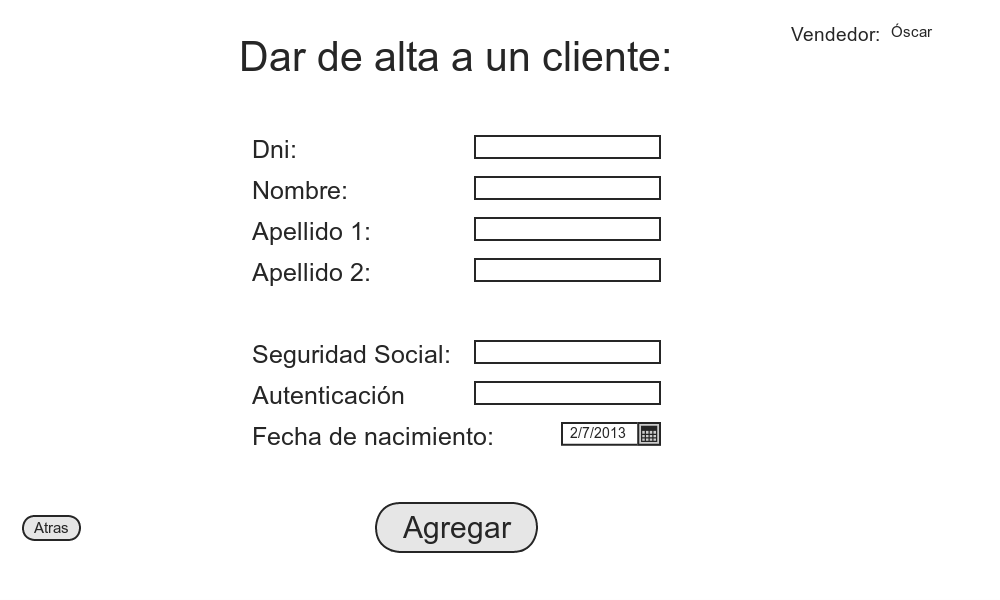
\includegraphics[width=0.8\textwidth]{Maquetas/AltaCliente.png}}
		\caption{Pantalla de alta de cliente: el vendedor introduce los datos necesarios del cliente para registrarlo en el sistema.} 
		\label{maqAltaCliente}
	\end{center}  
\end{figure}
\newpage
\printindex

\end{document}